\documentclass[defaultstyle,10pt,master]{thesis}
%!TEX TS-program = pdflatex
%!TEX encoding = UTF-8 Unicode

\usepackage[utf8]{inputenc} % set input encoding (not needed with XeLaTeX)

\usepackage[sort&compress,round]{natbib}
%\usepackage[square,numbers]{natbib}
\bibliographystyle{plainnat}
%\bibliographystyle{unsrtnat}

%for coloured hyperlinks
\usepackage{hyperref}
\hypersetup{ a4paper=true,
             colorlinks=false,
             citecolor=red,
             breaklinks=true,
             %bookmarks=true,
             bookmarksnumbered=true,
             bookmarksopen=true,
             pdftitle={Computational prediction of microRNA targets in plant genomes},                 % EDIT THIS LINE
             pdfauthor={Manuel Borges Dias dos Reis},                    % EDIT THIS LINE
             pdfsubject={Computational prediction of microRNA targets in plant genomes},                  % EDIT THIS LINE
             pdfcreator={Manuel Borges Dias dos Reis}, % EDIT THIS LINE
             pdfkeywords={miRNA, plants}                             % EDIT THIS LINE
}

%%% PAGE DIMENSIONS
\usepackage{geometry}
\usepackage{pdflscape}
\usepackage[T1]{fontenc}

\usepackage{graphicx} % support the \includegraphics command and options
\usepackage{caption}
\usepackage{subcaption}
\usepackage{wrapfig} % permite meter figuras no meio do texto

%% PACKAGE algorithmic, algorithm
%% ------------------------------
%% These packages are required if you need to describe an algorithm.
\usepackage{algorithmicx}
\usepackage{algorithm}
\usepackage[noend]{algpseudocode}
\usepackage{xspace}
\usepackage{setspace}
%\usepackage[chapter]{algorithm}

%\usepackage{citep}
\usepackage{float}
%\floatstyle{boxed}
%\restylefloat{figure}   % To re-style the 'figure' float
%\restylefloat{}    % To re-style the 'le' float.

%\usepackage[parfill]{parskip} % Activate to begin paragraphs with an empty line rather than an indent

\usepackage{pdfpages}

%%% PACKAGES
\renewcommand{\arraystretch}{1.2}
\usepackage{booktabs} % for much better looking tables
\usepackage{array} % for better arrays (eg matrices) in maths
\usepackage{paralist} % very flexible & customisable lists (eg. enumerate/itemize, etc.)
\usepackage{verbatim} % adds environment for commenting out blocks of text & for better verbatim
\usepackage{listings}
\usepackage{color}

\definecolor{codegreen}{rgb}{0,0.6,0}
\definecolor{codegray}{rgb}{0.5,0.5,0.5}
\definecolor{codepurple}{rgb}{0.58,0,0.82}
\definecolor{backcolour}{rgb}{0.95,0.95,0.92}

\lstdefinestyle{code}{
    backgroundcolor=\color{backcolour},
    commentstyle=\color{codegreen},
    keywordstyle=\color{magenta},
    numberstyle=\tiny\color{codegray},
    stringstyle=\color{codepurple},
    basicstyle=\footnotesize,
    breakatwhitespace=false,
    breaklines=true,
    captionpos=b,
    keepspaces=true,
    numbers=left,
    numbersep=5pt,
    showspaces=false,
    showstringspaces=false,
    showtabs=false,
    tabsize=2
}

\lstset{style=code}

%\usepackage{subfig} % make it possible to include more than one captioned figure/table in a single float
\usepackage[table]{xcolor}% http://ctan.org/pkg/xcolor
\usepackage[flushleft,para]{threeparttable}
\usepackage{tabularx}
\usepackage{tablefootnote}
\usepackage{changepage}
\usepackage{array}

\newcolumntype{L}[1]{>{\raggedright\let\newline\\\arraybackslash\hspace{0pt}}m{#1}}
\newcolumntype{C}[1]{>{\centering\let\newline\\\arraybackslash\hspace{0pt}}m{#1}}
\newcolumntype{R}[1]{>{\raggedleft\let\newline\\\arraybackslash\hspace{0pt}}m{#1}}


\newcommand{\HRule}{\rule{\linewidth}{0.5mm}}

% AMS packages
\usepackage{amsmath}
\usepackage{amsfonts}
\usepackage{amssymb}


%%%%%%%%%%%%%%%%%%%%%%%%%%%%%%%%%%%%%%
%%%%%%%%%%%%%%% FILIPA %%%%%%%%%%%%%%%
%%%%%%%%%%%%%%%%%%%%%%%%%%%%%%%%%%%%%%
\usepackage[printonlyused]{acronym}
\usepackage{todonotes}
\usepackage{graphicx}
\usepackage{subcaption}
\usepackage{pifont}
\usepackage{multirow}
\usepackage{array}
\newcolumntype{L}[1]{>{\raggedright\let\newline\\\arraybackslash\hspace{0pt}}m{#1}}
\newcolumntype{C}[1]{>{\centering\let\newline\\\arraybackslash\hspace{0pt}}m{#1}}
\newcolumntype{R}[1]{>{\raggedleft\let\newline\\\arraybackslash\hspace{0pt}}m{#1}}
\newcommand*{\Comb}[2]{{}^{#1}C_{#2}}
\normalem
%%%%%%%%%%%%%%%%%%%%%%%%%%%%%%%%%%%%%%
%%%%%%%%%%%%%%%%%%%%%%%%%%%%%%%%%%%%%%
%%%%%%%%%%%%%%%%%%%%%%%%%%%%%%%%%%%%%%

\usepackage{fixfoot,footmisc}

\usepackage{enumitem}

\newcommand*\BitAnd{\mathrel{\&}}
\newcommand*\BitOr{\mathrel{|}}

\algnewcommand\algorithmicinitialize{\textbf{Initialize:}}
\algnewcommand\Initialize{\item[\algorithmicinitialize]}

\algnewcommand\algorithmicbasis{\textbf{Basis:}}
\algnewcommand\Basis{\item[\algorithmicbasis]}

\algnewcommand{\Print}{\textbf{print}\xspace}
\algnewcommand{\Increment}{\textbf{Increment}\xspace}
\algnewcommand{\By}{\textbf{by}\xspace}
\algnewcommand{\BinAnd}{\textbf{and}\xspace}
\algnewcommand{\BinOr}{\textbf{or}\xspace}
\algnewcommand{\BitOr}{\mathrel{|}}

\hyphenation{microRNA} % allows defining the hyphenation of a particular work
\hyphenation{microRNAs}
\hyphenation{pre-miRNA}
\hyphenation{miRNA}
\hyphenation{miRNAs}

\hoffset 0in
\voffset 0in
\oddsidemargin 0.71cm
\evensidemargin 0.04cm
\marginparsep 0in
\topmargin -0.25cm
\textwidth 15cm
\textheight 23.5cm

\usepackage{fancyhdr}
\pagestyle{fancy}
\renewcommand{\chaptermark}[1]{\markboth{\thechapter.\ #1}{}}
\renewcommand{\sectionmark}[1]{\markright{\thesection\ #1}}
\fancyhf{} \fancyhead[LE]{\bfseries\nouppercase{\leftmark}}
\fancyhead[RO]{\bfseries\nouppercase{\rightmark}}
\fancyfoot[LE,RO]{\bfseries\thepage}
\renewcommand{\headrulewidth}{0.5pt}
\renewcommand{\footrulewidth}{0.5pt}
\addtolength{\headheight}{2pt} % make space for the rule
\fancypagestyle{plain}{%
   \fancyhead{} % get rid of headers
   \renewcommand{\headrulewidth}{0pt} % and the line
   \renewcommand{\footrulewidth}{0pt}
}
\fancypagestyle{blank}{%
   \fancyhf{} % get rid of headers and footers
   \renewcommand{\headrulewidth}{0pt} % and the line
   \renewcommand{\footrulewidth}{0pt}
}
\fancypagestyle{abstract}{%
   \fancyhead{}
   \renewcommand{\headrulewidth}{0pt}
   \renewcommand{\footrulewidth}{0.5pt}
}
\fancypagestyle{document}{%
	\fancyhf{} \fancyhead[LE]{\bfseries\nouppercase{\leftmark}}
	\fancyhead[RO]{\bfseries\nouppercase{\rightmark}}
	\fancyfoot[LE,RO]{\bfseries\thepage}
	\renewcommand{\headrulewidth}{0.5pt}
	\renewcommand{\footrulewidth}{0.5pt}
	\addtolength{\headheight}{2pt} % make space for the rule
}
\setcounter{secnumdepth} {5}
\setcounter{tocdepth} {5}
\renewcommand{\thesubsubsection}{\thesubsection.\Alph{subsubsection}}


%for submmited but yet to be accepted publications
\newcommand{\noop}[1]{}
\begin{document}



\pdfbookmark[0]{EMYS: A Social Robot that Plays ``Sueca''}{Title}

\univlogo{1.2cm}{0.5cm}{img/logo_ist}

%\thesislogo{2.9cm}{6.4cm}{report_pictures_tables/eucalyptus-triplet-photo.pdf}

\title{EMYS: a social robot that plays ``Sueca''}

\author{Filipa Isabel Nogueira Correia}

\degree{Information Systems and Computer Engineering}

\supervisor{Prof. Dr.  Ana Maria Severino de Almeida e Paiva}
\othersupervisor{Prof. Dr. Francisco António Chaves Saraiva de Melo}

\date{November 2015}

\finalthesis{true}

\presidentofjury{Prof. Dr. João Emílio Segurado Pavão Martins}
\vogalone{Dr. Manuel Fernando Cabido Peres Lopes}



\maketitle %produces the title
\thispagestyle{empty}
\cleardoublepage
\setcounter{page}{1}
\pagenumbering{roman}

\baselineskip 18pt % line spacing: -12pt for single spacing
                   %               -18pt for 1 1/2 spacing
                   %               -24pt for double spacing

\pdfbookmark{Acknowledgments}{Acknowledgments}
\begin{acknowledgments}

I would like to thank...

\end{acknowledgments}
\pdfbookmark{Abstract}{Abstract}
\begin{abstract}

Regarding the needs of elder population, technology can be the answer to some of them.
Existing robots already guide the elderly walking through the house, or are companions for cuddling and petting. In the same way, this work aims to create a companion robot that plays the card game \emph{Sueca}. The idea is to develop an entertaining and pleasuring environment that can, additionally, stimulate their reasoning.
After reviewing the related work, this report proposes an artificial player based on Monte-Carlo methods and the architecture that will use it. Considering the game state, the chosen move, and some of the environment perceptions, this robot must produce an appropriate behaviour to be considered socially present during the game.


\end{abstract}

\begin{keywords}
Artificial Intelligence, Trick-taking Card Game, Hidden Information, Interactive Companions, Socially Intelligent Behaviour
\end{keywords}
\clearpage
\thispagestyle{empty}
\cleardoublepage

\pdfbookmark{Resumo}{Resumo}
\begin{resumo}

A complexidade computacional de alguns jogos de cartas atrai o interesse de investigadores na área da Inteligência Artificial.
Apesar do maior desafio ser a informação escondida, já existem algumas abordagens capazes the ultrapassar este problema, tais como metodologias baseadas em Monte-Carlo.
Por outro lado, a componente social que os jogos com multijogadores apresentam é bastante forte e pode, no entanto, ser incluída num jogador artificial através de roboôs que interagem com os outros jogadores.
Deste modo, esta tese propõe o desenvolvimento de um jogador social de Sueca que é capaz de jogar o jogo enquanto comunica com jogadores humanos, melhorando a experiência do jogo.
Este agente incluiu um módulo de IA capaz de decidir que carta jogar, com base no algoritmo \emph{Perfect Information Monte-Carlo}.
Para além disso, de maneira a estar socialmente presente durante o jogo, este agente também contém um módulo de decisão capaz de avaliar o estado do jogo e de produzir comportamentos verbais e não verbais adequados.
Por fim, estudos com utilizadores revelaram comparações significativas com jogdares humanos, incentivando o futuro desenvolvimento deste trabalho.
\end{resumo}

\begin{palavraschave}
Artificial Intelligence, Trick-taking Card Game, Hidden Information, Interactive Companions, Socially Intelligent Behaviour
\end{palavraschave}

\clearpage
\thispagestyle{empty}
\cleardoublepage

\dominitoc
\dominilof
\dominilot

\pdfbookmark[0]{Index}{index}
\pdfbookmark[1]{Contents}{toc}
\tableofcontents
\cleardoublepage
\renewcommand{\baselinestretch}{1.5}

\pdfbookmark[1]{List of Figures}{lof}
\listoffigures
\cleardoublepage

\pdfbookmark[1]{List of Tables}{lot}
\listoftables
\cleardoublepage

\pdfbookmark[1]{Glossary}{loac}
\renewcommand{\listofacronymsname}{Glossary}
\listofacronyms

\begin{acronym}[PIPMA]
\acro{emys}[EMYS]{EMotive headY System}
\acro{hci}[HCI]{Human-Computer Interaction}
\acro{hri}[HRI]{Human-Robot Interaction}
\acro{vhri}[VHRI]{Video-based HRI}
\acro{thri}[THRI]{Theatre-based HRI}
\acro{ai}[AI]{Artificial Intelligence}
\acro{qa}[QA]{Question Answering}
\acro{mcts}[MCTS]{Monte-Carlo Tree Search}
\acro{uct}[UCT]{Upper Confidence Bounds for Trees}
\acro{pimc}[PIMC]{Perfect Information Monte-Carlo}
\acro{ismcts}[ISMCTS]{Information Set Monte-Carlo Tree Search}
\acro{iimc}[IIMC]{Imperfect Information Monte-Carlo}
\acro{gib}[GIB]{Ginsberg's Intelligent Bridgeplayer}
\acro{pipma}[PIPMA]{Perfect Information Post-Mortem Analysis}
\acro{csp}[CSP]{Constraint Satisfaction Problem}
\end{acronym}

\cleardoublepage




\setcounter{page}{1} \pagenumbering{arabic}
\baselineskip 18pt
\cleardoublepage

\fancychapter{Introduction}
\section{Introduction}
\label{sec:introduction}

The world population is ageing dramatically and as such, the society needs to change and embrace this problem in many different ways. The elderly have specific needs, physical and cognitive, that are often not considered in the way we, as a society, organise our lives.  
Some of these concerns are recently being solved with the help of technology and may range from computer programs to intelligent robots.
For instance, elderly with mobility disabilities may be guided by a robot while walking through the house \cite{Pollack2002}.
Another example is software for stimulating and training memory problems of Aphasia, a language disorder caused by brain damage \cite{Pompili2011}.

However, existing technology with elderly purposes is commonly focused on health care.
When dealing with aged people with no serious health problems and that are still capable of doing their regular daily tasks, there is still a need to occupy their free time with pleasuring activities.
Finding appropriate tasks supported by technology may include the training of their cognitive functions or just accompany them.
In order to join these two purposes of accompany and train their reasoning, an artificial game player could be a suitable solution.
Several embodied agents for game playing exist, such as the iCat chess tutor \cite{Affective2007} and the \ac{emys} Risk player \cite{Pereira}.%, nevertheless these scenarios were not applied to aged people.
These examples have inspired the idea of exploring a card game scenario, that can exemplify an activity that aged people enjoy doing.
%Several embodied agents for game playing exist, such as the iCat chess tutor \cite{Affective2007} and the \ac{emys} Risk player \cite{Pereira}, nevertheless these scenarios were not applied to aged people.

Overall, a card game is an entertainment activity that aged people are used to do and, at the same time, might help them training their cognitive functions.
As a result, considering some of existing card games are still unsolved challenges for \ac{ai}, the goal of this project is to integrate a social robot with aged humans in a card game scenario.
This project is a great opportunity to relate all the concerns mentioned above.
%On one hand, the proposed agent should play the game correctly, which means, after analysing the given hand, dealt at the beginning of the game, it should make good choices about what cards should be played.
%On the other hand, this embodied agent should act accordingly to the environment of this scenario and every player should be engaged in the game with its interaction and behaviours.
A game-playing companion for elder people must, at the same time, (i) be able to play competently the card game; and (ii) interact socially. The first skill requires such agent to include an AI module that is able to reason strategically about the game. The second skill requires an emotional/social module that enables the agent to behave in a manner that is socially believable.


Computer programs that play games have been an interesting challenge for \ac{ai}.
From board to card games, or even role-playing games, the goal is to create rational agents capable of evaluating the game and achieving the best outcome.
Deep Blue, Chinook and Watson are good examples that have raised the bar for developing this kind of agents.
Deep Blue is a remarkable chess player and has defeated the human world champion in 1997 \cite{Campbell2002}.
Schaeffer et al. have solved Checkers with Chinook program and proved the game leads to a draw with two optimal players \cite{Schaeffer1996}.
Lastly, Watson is the \ac{qa} system that has beat the two highest ranked Jeopardy players in 2011 \cite{Ferrucci2010}.
%\ac{qa} systems are extremely impressive due to the scope of \ac{ai} they include (i.e. natural language processing, machine learning, knowledge representation, automated reasoning, and information retrieval).
All these agents are good baselines to improve \ac{ai} in games.


Besides building programs that try to think rationally or humanly, \ac{ai} has also another branch that aims to act humanly \cite{Russell2009}.
This concern arises from the inclusion of robots in humans' life and influences the way they interact and communicate with people.
Consequently, robots have to behave properly in those environments, considering they are surrounded by humans.
The \ac{hri} field explores these concerns of integrating robots with humans in a social environment.
Since this field descends from \ac{hci}, it also inherits the user centred development that establishes the prior need of doing user studies.


%Consequently, technology that covers this point has concerns related with the feeling of objectification, loss of responsibilities and privacy \cite{Should2010}.



Lastly, the chosen card game is \emph{Sueca}, a well known Portuguese game among the ageing population.
It is a four-player game with two teams and involves an opponent and a companion role for the agent.
Regarding \ac{hri} concerns, these two roles together have not been studied yet in an artificial embodied game player.



\subsection{Goals}
\label{sec:goals}

The main goals of this project are:
\begin{itemize}
\item To develop a robotic agent capable of playing competently the \emph{Sueca} card game;
\item To include social behaviours on an embodied agent in order to act according to the game state;
\item To evaluate the correctness and advantages of the proposed system.
\end{itemize}

\subsection*{\centering*}

The next section presents some background research that helps the reader understand the problems further mentioned (Section~\ref{sec:background}).
The report proceeds with the state-of-art of playing card-games and human-robot-interaction with the elderly (Section~\ref{sec:related-work}).
Additionally, it reveals a pilot user study (Section~\ref{sec:user-studies}).
Finally, it presents the architecture, its evaluation methodology and the final conclusions.

\fancychapter{Background}
\label{chapter:background}

The current section introduces the discussion of relevant research in order to understand some concepts and terminology further mentioned.

\subsection{Game theory concepts}

Game theory studies decision making problems involving multiple decision makers.
A problem of this nature is usually called a game and defines a set of constraints to the players' actions.
It also studies the strategies these players might take and the properties of each game.
%This subject is applied to many different areas, such as economics, political science, biology, or computer science.

Each decision maker tries to maximise the payoff/reward of his possible actions and one possible approach to do that is to consider the opponents' actions.
The Nash-equilibrium \cite{Nash1950} of a game is a stable strategy for every player and occurs when each player chooses the best strategy for himself, considering their opponents have the same behaviour.
Moreover, each player cannot have a better benefit by changing his strategy unilaterally.

\begin{figure}
\centering

\includegraphics[width=1\textwidth]{./img/gamesHierarchy}
\caption{Hierarchy of games}
\label{fig:games}
\end{figure}

Figure~\ref{fig:games} shows how games can be hierarchically categorised \cite{Osborne2011}.
In a cooperative game, players cooperate with one another in order to achieve a common goal.
Alternatively, in a non-cooperative game, each player works independently for its own purposes.
Non-cooperative games can also be branched into two forms: normal and extensive form \cite{Shoham2010}.
A normal form game can be defined as the tuple $(N,(A_k)_{k=1}^{N},(u_k)_{k=1}^{N})$, where:

\begin{itemize}
\item $N$ is the number of players;
\item $A_k$ is the finite set of available actions for the $k$-th player;
\item $u_k$ is the payoff for the $k$-th player.
\end{itemize}

Additionally, considering the players' payoffs, another relevant concept is the zero-sum game, where the sum of all players' payoffs is zero.
For instance, in a zero-sum 2 players game, $u_1 = -u_2$.
Although the normal form games assume that players' actions are made simultaneously, in the extensive form games, the players' actions are sequential.
This evidence leads to another branching in the hierarchy of games and, consequently, an extensive game can be considered as a perfect information and an imperfect information game.
In perfect information games, each player knows exactly the real state of his opponents, (e.g. Chess).
%The second means opponents' state is hidden (e.g. Poker).
In imperfect information games, the game state is not fully observable to the players. For instance, in a Poker game, a player only knows its own cards, the cards in the table, and the bets of all players. 

In imperfect information games, an \emph{information state} or \emph{information set} for a player $k$ corresponds to a set of all games states that yield the same “observation” to player $k$. For example, in a Poker game, an information set consists in all game-states that lead to the same observed cards in the table and in the player’s hand.

%Considering the focus of this work on a card game, another relevant point on top of hidden information games is the definition of information set.
%An information set aggregates several nodes representing unknown information such as choice nodes. In a card game, for instance, the information set of a player, whose cards are hidden, corresponds to all the possible combinations of his hand.




\section{The game of \emph{Sueca}}
\label{sec:sueca}

\emph{Sueca} is a card game categorised as trick-taking, which means the game has a finite number of rounds, called tricks.
In this case, there are ten tricks, since the deck has forty cards equally distributed among the four players.
This game uses the standard French card deck, excluding the rank 8 through 10.
Although most trick-taking card games count the number of winning tricks to determine the winner, \emph{Sueca} assigns points to the cards, according to Table~\ref{tab:points-table}.
The most significant difference, compared to other games, is the card with rank 7 being higher than the King (K) and lower Ace (A).


All valued cards sum 120 points, which means a team with more than 60 points wins the game.
Moreover, each player is paired with the player in front of him, and the two adjacent players form the opposing team.
Hence, the game involves both cooperation and competition.

\begin{table}[ht]
\centering
\caption{Rank of cards per suit and respective reward values}
\begin{tabular}{|C{0.1\textwidth}|C{0.1\textwidth}|C{0.1\textwidth}|C{0.1\textwidth}|C{0.1\textwidth}|C{0.1\textwidth}|C{0.1\textwidth}|}
\hline
\textbf{Cards}  & 2-6 & Q & J & K & 7  & A\\
\hline
\textbf{Points} & 0   & 2 & 3 & 4 & 10 & 11\\
\hline
\end{tabular}
\label{tab:points-table}
\end{table}

After the deck has been shuffled and divided, the dealer chooses the top or bottom card to be the trump suit, leaves it on the table, and distributes the remaining cards among all players.
The remaining rules are quite similar to any other trick-taking games:
\begin{itemize}
\item Follow the suit of the first card played in the turn (lead suit), if possible;
\item A player wins the trick if his card has the highest value belonging to the lead suit or the trump suit.
\end{itemize}


\emph{Sueca} is a nondeterministic game, since it includes what is called the element of chance by the cards being dealt randomly at the beginning.
Additionally, since the cards of each player are hidden from the other players, this is considered as an imperfect information game.
There are almost $1.9\times10^{22}$ possible card distributions\footnote{$4\times\Comb{40}{10}\times\Comb{30}{10}\times\Comb{20}{10}$}.
%Nevertheless, considering the initial hand of the agent, the uncertainty about other players' hands decreases to $5.9\times10^{12}$ \footnote{$\Comb{30}{10}\times\Comb{20}{10}$}.
\subsection{Monte-Carlo Tree Search}


\ac{mcts} is a family of algorithms whose goal is finding optimal decisions, by combining standard tree search with Monte-Carlo sampling \cite{Browne2012}.
This method incrementally builds a search tree according to the results of previous iterations.
The search tree is expanded by randomly sampling the nodes.
Usually, it is divided into four steps, as described below.
\begin{itemize}
  \item Selection: To select a child node through a selection policy. This policy must balance between unexplored areas of the tree and promising nodes that may lead to higher rewards.
  \item Expansion: To expand the selected node to add one or more nodes to the tree, according to the available actions.
  \item Simulation: To select an expanded node through a simulation or default policy to produce an outcome.
  \item Backpropagation: To propagate the reward value of all the selected nodes in order to update their statistics.
\end{itemize}


The main strength of \ac{mcts} is its little knowledge requirement, and so, it can be applied to many different domains.
This algorithm can also be easily paralleled, since each simulation process can be done independently.


According to Browne et al., finding a suitable variation of \ac{mcts} is the greatest challenge of applying the algorithm to a specific environment.
The most popular algorithm of \ac{mcts} family is \ac{uct}, and this variation differs from the original in the selection phase.
It uses a maximisation function to evaluate the available nodes, according to the following equation:

\begin{equation}
    UCT = \overline{X}_j + c\sqrt{\frac{\ln n}{n_j}},
\end{equation}

where $\overline{X}_j$ represents the average value associated with option $j$ in the current state, $n_j$ is the number of times that option $j$ was selected in the current state, $n$ is the number of visits to the current state and $c$ is an exploration parameter.

It models the reward of each child node as an independent multiarmed bandit problem.
This means that, besides considering the already obtained average reward of a child node ($\overline{X}_j$), it also considers the maximum expected gain of that same child node ($c\sqrt{\frac{\ln n}{n_j}}$).
This function establishes an equilibrium between exploitation and exploration.
Exploitation is evaluated in the first term of the equation by considering the average reward of a child node.
The exploration is manipulated in the second term by balancing the amount of times the parent node and the child node $j$ have been visited (respectively, $n$ and $n_j$).
A considerable amount of iterations will approximate the \ac{uct} to a minimax tree.
Consequently, the produced results are nearly optimal with high probability.

 

\fancychapter{Related work}
\label{chapter:related-work}

This chapter presents the state of the art related to this work.
Since no relevant studies on \emph{Sueca} have been found, the research is focused on algorithms used in similar card games.
It also presents existing companion and game-player robots that will allow the analysis on human-robot interaction relevant for this work.


\section{AI in games}

%%% jogos tem sido um grande desafio
\ac{ai} has been solving many games over the years, however, the definition of "games" usually refers to zero-sum and perfect information games.
These kind of games are commonly solved by creating a tree representing all possible states and searching for the optimal, or a nearly optimal, solution.
The greatest achievements related to perfect information games are generally based on finding good heuristics to refine the search and also good prunings to reduce the search space.
Deep Blue can exemplify this idea \cite{Campbell2002}, it uses an iterative-deepening alpha-beta search and the key of its success is mostly the null move heuristic and the futility pruning.
Another example is Chinook, also a perfect information game that was solved using alpha-beta search \cite{Schaeffer1996}.

%%% perfect e imperfect nao se resolvem da mesma maneira
Nevertheless, \emph{Sueca} is considered an imperfect information game, as described in Section~\ref{sec:background}, and this class of games is usually solved by one of three different approaches \cite{Cowling2012}.
The first one, and the most popular, is based on Monte-Carlo Methods.
Then, another possible approach is trying to compute a Nash equilibrium strategy or an approximation thereof.
Lastly, belief distributions involving game state inferences and opponent models can also be used.
The first two mentioned approaches are mutually exclusive, while the last one can be used as a supplement.
The following two subsections detail how Monte-Carlo Methods and Belief Distributions can be applied in hidden information games.
The second pointed approach will not be addressed due to the imposed limitations of our domain, considering, for instance, that the maximum known number of states for computing a Nash equilibrium is $10^{12}$ \cite{Zinkevich}, which is much lower than the number of possible states in a \emph{Sueca} game.




\subsection{Monte-Carlo Methods}

%%% monte carlo e cada vez mais popular
The popularity and acceptance of Monte-Carlo based methods have increased since its success on Bridge.
\ac{gib}\footnote{http://www.gibware.com/} was the first computer bridge champion using Monte-Carlo Methods, and subsequently, another two successful domains were Skat\footnote{https://skatgame.net/} and Computer Go \cite{Gelly2011}.
Since some of these domains remain a challenge for traditional \ac{ai} techniques, this method seems to be very promising.


%%% diferenca entre MCTS e PIMC
In order to solve a hidden information game, the first challenge is to deal with information sets.
The most used approach to solve it is determinization, which samples choice nodes instead of considering all of them in an unique set.
Applying this approach to \ac{mcts} is known as \ac{pimc}.
For instance, in a card game scenario, each iteration of \ac{pimc} samples the cards distributions for all players and the simulation process of the game behaves as a perfect information game.
In other words, during the simulation each player makes decisions as if his opponents' cards are visible.
The first successful implementation of this technique was \ac{gib} \cite{Ginsberg2001}.


%%% Basin estudou os prblomeas do PIMC
In 1998, Frank \& Basin produced an analysis on \ac{pimc}'s limitations \cite{Frank1998}.
They identified two distinct problems: \emph{strategy fusion} and \emph{non-locality}.
Due to the repeated minimaxing architecture that \ac{pimc} has and its evaluation of possible distributions with the best strategy, applying this knowledge, when information is missing, might produce suboptimal decisions.
This is called the \emph{strategy fusion}.
For instance, when having a move with a guaranteed reward and another move with a possible reward of the same value although depending on the current world, \ac{pimc} equally considers both moves.


The second problem, \emph{non-locality}, results from the propagation of values.
The value of a game tree node only considers its children' values, however, in an imperfect information game, some guesses might be done using values of the non-local subtree.
For instance, considering 2 different worlds, the player 1 can guarantee a winning trick in the world 1 by making a certain move, and if in that state, he makes another move instead, player 2 might assume they are in world 2.
\ac{pimc} cannot make such an inference.


%%% O Long estudou com que propriedades o PICM funciona
Despite the satisfying outcomes of \ac{pimc}, there were still difficulties in understanding the strong results of this algorithm.
As such, Long et al. have analysed the previously mentioned problems of \ac{pimc} search, and they have shown how three different properties of a game can influence the success of \ac{pimc} \cite{Long2010}.
The first property is \emph{leaf correlation}, which refers to how likely it is to affect a player's payoff in the neighbourhood of a leaf.
When the probability of all siblings having the same payoff values is higher, the correlation value increases.
Secondly, \emph{bias} indicates the chance of a player being preferred over another.
Finally, the last game characteristic that has been pointed is \emph{disambiguation factor}, that denotes how rapidly the hidden information is revealed.


These properties have been tested in a set of experiments in both \ac{pimc} and a random player against an optimal Nash equilibrium player.
Results shown the performance of \ac{pimc} increases as the correlation value is higher, bias does not considerably affect its success, and, finally, disambiguation has the greatest impact on the results of the algorithm.
When this last value is higher, it means the game turns more quickly into a perfect information game.
Additionally, the authors demonstrate these properties on real game examples, such as Skat and Kuhn poker.
Skat indicates a considerably good performance of \ac{pimc}, due to its values of \emph{leaf correlation}, \emph{bias}, and \emph{disambiguation factor}.
Since Skat presents strong similarities to \emph{Sueca}, it is expected that \ac{pimc} also has a good performance when applied to \emph{Sueca}.


%%%  cowling propose ISMCTS
Cowling et al. have also investigated the application of \ac{mcts} to hidden information games \cite{Cowling2012}.
Their research supports a new descendant family of algorithms, \ac{ismcts}.
\ac{ismcts} works with information sets, instead of game states and uses determinization to sample the game, however producing a single tree.
The main advantages are the computational budget efficiency and the fact of suffering less from \emph{strategy fusion} than \ac{pimc}.
The authors also presented some experiments in three different games, including a card game.
Their results on the card game Dou Di Zhu were very similar to \ac{uct} and did not introduce any improvement to the playing strength.
The authors explained these results with the high branching factor this domain produces, which has discouraged the usage of this technique on the domain of \emph{Sueca}, since in the information set tree, the initial branching factor would also be high ($10^{8}$, $\Comb{40}{10}$).


%%% IIMC
Recently, Furtak \& Buro \cite{Furtak} presented a new search algorithm called \ac{iimc} that can be suitably applied to hidden information games and reduces the \emph{strategy fusion} problem.
During the simulation phase, each player's move is chosen inside a player's module and the game behaves as an imperfect information due to this encapsulation.
Additionally, the players' modules allow the differentiation of players using different strategies.
The authors revealed the great potential of this approach when applied to trick-based card games, considering it has been successfully tested in the Skat scenario.


\begin{table}[h]
\caption{Advantages and disadvantages of the mentioned Monte-Carlo algorithms}
\resizebox{\textwidth}{!}{%
\begin{tabular}{|c|l|l|}
\hline
\textbf{Algorithm} & \multicolumn{1}{c|}{\textbf{Advantages}} & \multicolumn{1}{c|}{\textbf{Disadvantages}}\\
\hline
\ac{pimc}      & \begin{tabular}[c]{@{}l@{}}Offline Computation\\ Easy to parallel\end{tabular}                                             & \begin{tabular}[c]{@{}l@{}}Strategy fusion\\ Non-locality\end{tabular}                                        \\ \hline
\ac{ismcts}    & \begin{tabular}[c]{@{}l@{}}Offline Computation\\ Easy to parallel\\ Computational budget\end{tabular}                      & \begin{tabular}[c]{@{}l@{}}Strategy fusion (less than \ac{pimc})\\ Non-locality\\ Complexity\end{tabular}                       \\ \hline
\ac{iimc}      & \begin{tabular}[c]{@{}l@{}}Offline Computation\\ Easy to parallel\\ Allow a different player model per player\end{tabular} & \begin{tabular}[c]{@{}l@{}}Strategy fusion (less than \ac{pimc})\\ Non-locality\\ Complexity\end{tabular} \\ \hline
\end{tabular}
}
\label{tab:algorithms}
\end{table}


%Due to the similarity between \emph{Sueca} and Skat, it is predictable that Monte-Carlo methods might produce good results in our domain.
%However, assuming that different \ac{mcts} variations produce the exact same behaviour, in different domains, might be a mistake, considering they have specific characteristics. % esta errado

The advantages and disadvantages of the mentioned \ac{mcts} variations are clearly summarised in Table~\ref{tab:algorithms}.
Both of three techniques are easy to parallel and allow an offline computation. However, \ac{ismcts} uses the computational budget more efficiently than the other two techniques, and \ac{iimc} allows different player models per player.
Disadvantages show all the three techniques have the \emph{non-locality} and \emph{strategy fusion} problem, although \emph{strategy fusion} is lower in \ac{ismcts} and \ac{iimc}.
Another relevant disadvantage is the computational burden that \ac{ismcts} and \ac{iimc} add, when compared to \ac{pimc}.
%Despite having a better computational budget, applying \ac{ismcts} to \emph{Sueca} should produce a similar behaviour to Dou Di Zhu, due to the high branching factor in the information set tree.
%The usage of different player models can be helpful to turn the game to an imperfect information game and, consequently, reduce the \emph{strategy fusion} problem.







\subsection{Game State Inference \& Opponent Modelling}


While discussing imperfect information games, belief distributions, game state inference and opponent modelling are another relevant subjects to consider.
Predicting some of the opponents' cards or other clues would be beneficial to select better actions at each state of the game. Additionally, inferring hidden information, while using a Monte-Carlo based method, can also decrease the \emph{non-locality} problem \cite{Cowling2012}.
%This problem is known as finding the distribution $P$(world\textbar move) for a move played in an hypothetical world.


Buro in 2009 \cite{Buro} presented his work on state evaluation and inference that has been included in his Skat player.
His approach combines two techniques, one for evaluating the bidding and another for selecting hypothetical worlds during the game play.
The former technique uses a logistic regression to evaluate the winning probability of each hand and it has 22 million Skat games as data base.
This winning probability determines the strength of a hand and can, therefore, be used on the bidding.


The second technique is mainly based on two heuristics.
Fastest-cut-first search heuristic evaluates each move according to its beta-cutoff value and minimises the expected number of visited nodes.
Additionally, in order to reduce the tree exploration, another heuristic groups cards by their strength value and considers, for example, 7\ding{168} and 8\ding{168} the same move, when holding both cards in a player's hand.
The author compares his work to other similar ones and concludes the strength of his techniques lies in two central points.
First, determining the $P$(world\textbar move) on offline data, instead of doing it in runtime.
Sencond, his formulation is generalised in a way that it is possible to perform it on high-level features.
Since the main difference between \emph{Sueca} and Skat is that the first one does not have the bidding phase, Buro's first technique would not be appropriate for the \emph{Sueca} game.
However, the search enhancements could be suitably applied, considering the game trees are identical.


Usually, opponent modelling uses optimal strategies to predict the other players' actions and these models tend to be overly defensive.
Consequently, Long \& Buro in 2011 \cite{Long2009} suggested a post-processing analysis that is able to infer opponent's qualities based on their decisions in a certain environment.
The main idea is to classify each opponent with a mistake rate and use that value to be more or less defensive.
This approach, called \ac{pipma}, computes a procedure after each game episode (in a trick-taking card game, it would be after each trick) to incrementally update the mistake rate of each opponent.
The authors made some experiments in a Skat player with very good results, where they used the mistake rate to adjust the bidding behaviour during the game.
%Likewise, the search improvements reduced about 40\% of the search space.
Despite the fact that \emph{Sueca} does not have the bidding phase, classifying opponents with a mistake rate can useful to other purposes.
As a result, it would be interesting to model the opponents in a similar way in the domain of \emph{Sueca}, in order to make better decisions or even for the embodied agent to produce adequate behaviours.

Another highly suitable card game to make opponent models is Poker, since predicting the players' moves can naturally affect the outcome of this game.
In order to predict players' cards and their future actions, Posen et al. in 2010 \cite{Ponsen2008} have investigated this subject.
They proposed an opponent model that starts with a prior distribution and changes over time with a differentiating function.
The prior distribution allows it to make reasonable inferences while having insufficient information.
In addition, the relational probability tree algorithm TILDE builds a decision tree with the stored samples of a player.
This decision tree represents the differentiating function that will adapt the initial prior distribution.
Besides this opponent model, the authors explain how to integrate this function with \ac{mcts}.
Instead of sampling the cards randomly, \ac{mcts} uses card predictions and, therefore, the algorithm does not need a numerous amount of iterations to reach a uniform card distribution.
Furthermore, the probabilities of action predictions are used in the selection phase of the \ac{mcts}, according to the state of the game and the sampled cards.
Since \ac{mcts} can be used in the \emph{Sueca} domain, a similar opponent model can also improve the capabilities of this algorithm, as shown in Poker.




\begin{table}[h]
\caption[Reviewed techniques and their goals]{Techniques signed with \ding{53}, \ding{51} and $\sim$ symbols are, respectively, not suitable, suitable and conditionally suitable to the \emph{Sueca} domain.}
\resizebox{\textwidth}{!}{%
\begin{tabular}{|C{0.1\textwidth}|l|l|C{0.12\textwidth}|}
\hline
\textbf{Tested domain} & \multicolumn{1}{c|}{\textbf{Technique}}     & \multicolumn{1}{c|}{\textbf{Goal}} & \textbf{Suitable to \emph{Sueca}} \\ \hline
\multirow{4}{*}{Skat}  & Determine the winning probability of a hand & Improve the bidding                & \ding{53}                         \\ \cline{2-4}
                       & Fastes-cut-first heuristic                  & Order moves                        & \ding{51}                         \\ \cline{2-4}
                       & Considering similar states equally          & Reduce tree exploration            & \ding{51}                         \\ \cline{2-4}
                       & Calculate the mistake rate of each player   & Improve the bidding                & $\sim$ \\ \hline
Poker                  & Opponent model                              & Improve \ac{mcts} policies      & \ding{51}                         \\ \hline
\end{tabular}
}
\label{tab:belief}
\end{table}



Table~\ref{tab:belief} summarises what techniques have been reviewed, their purposes, and, finally, if they can be applied to the \emph{Sueca} domain.
The technique of determining the winning probability cannot be used for the exact same purpose, since our domain does not include a bidding phase.
The next two search enhancements can naturally be used due to the similarities between Skat and our domain game trees.
The mistake rate was signed as conditionally suitable because it can also be used, although with a different purpose.
Thinking in the embodied agent of our work, it can assign a mistake rate variable to each player and produce appropriate behaviours according to their values.
A similar approach might be thought to use the winning probability, however, opponents' hands are not visible and the agent should not reveal its own information.
The last technique also can be an addition to the \ac{mcts} base policies.



\section{Human-robot interaction}

Regarding the goals of this project, it is crucial to investigate and evaluate the state of the art of \ac{hri}, in particular in the context of robot companions or players.
Since it aims to interact with aged people in a card game scenario, there are two clear branches that must be studied.
Firstly, the existing robots with an elderly care purpose.
Secondly, how social agents have been integrated into games.
The next subsections will address these points.
\todo[inline]{review this introductory text and get the focus on social robots in games}


\subsection{Social robots in games}

\todo[inline]{review this subsection and find more related work!!!!!!!!!!!!!!}
The idea of entertainment robots, which was previously mentioned, is expanding and becoming more frequent.
Its general goal is to create a social robot to interact with humans through a specific entertainment activity.
These activities should be lifelike experiences providing pleasure and enjoyment feelings.
Depending on the target audience, they can also be included in more challenging or even pedagogic activities.

Leite et al. uses the \emph{iCat} robot in a chess game scenario with children \cite{Castellano2010,Leite,Leitea}.
This chess companion also has the role of a tutor due to the help it provides during the game, for instance, it expresses opinions about children' moves so that they can improve their chess skills.
After their first pilot studies, the authors revealed the need of including social and cognitive abilities, commonly referred as empathy.
Their further studies introduced into the \emph{iCat} affect recognition in order to improve the robot's social cues.
The way they address this point includes recognising users' expressions and considering others' affective states.
For instance, when a child is losing, the \emph{iCat} comments about his moves should not cause embarrassment.
In addition, and considering their goals were also focused on long-term interactions, this chess player recognises faces and greet people mentioning past events.

This agent has some similarities and differences with the proposed agent of this work.
On one hand, including empathic behaviour to robots usually leads to more engaging, natural and likable experiences to users.
On the other hand, the \emph{iCat} in this scenario needs access to more details of users' emotional state because of its tutoring advices. Our \emph{Sueca} player will not advise other players about their actions, instead it will comment the game state.
Additionally, the target audience is clearly different and may lead to different concerns, and their work was also focused on long-term interaction.


\begin{figure}[h]
        \centering
        \begin{subfigure}[h]{0.48\textwidth}
                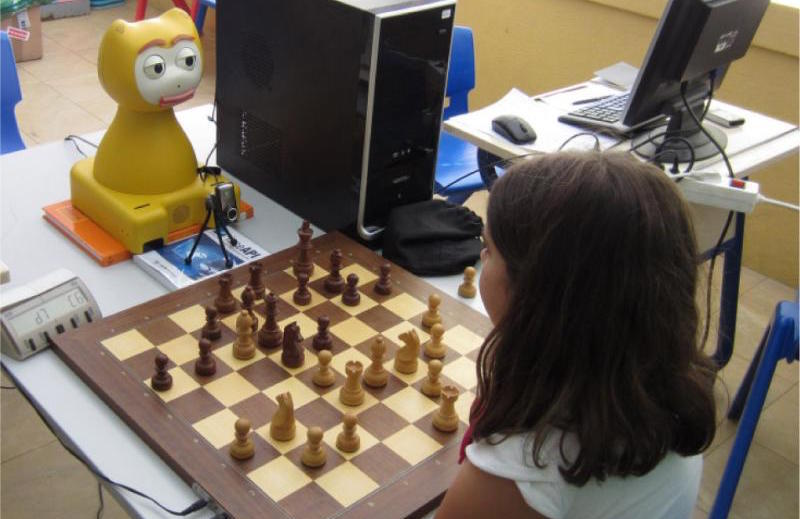
\includegraphics[width=\textwidth]{./img/icat}
                \caption{iCat - Chess tutor}
                \label{fig:icat}
        \end{subfigure}
        \begin{subfigure}[h]{0.5\textwidth}
                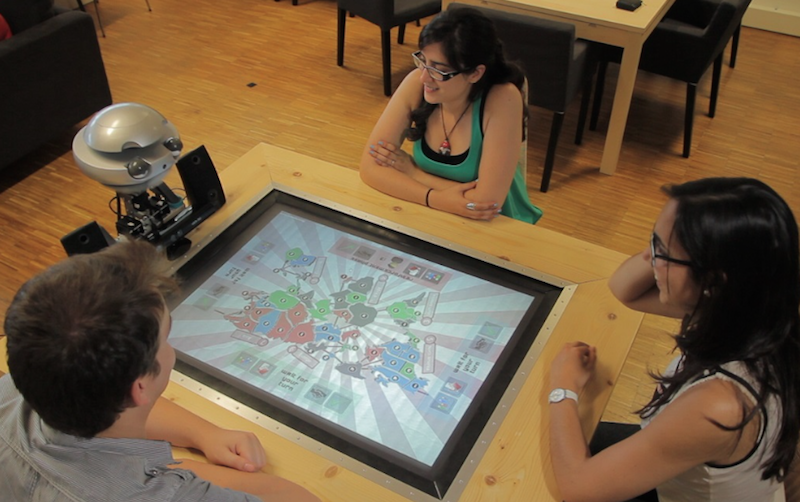
\includegraphics[width=\textwidth]{./img/emys}
                \caption{EMYS - Risk player}
                \label{fig:emys}
        \end{subfigure}
        \caption{Companion robots in game playing scenarios.}\label{fig:game-robots}
\end{figure}


Another example of a robot integrated into a game scenario is the Risk player by Pereira et al. \cite{Lisboa}.
The goal of their work was to create a robot that interacts with humans and is perceived as socially present in long-term interactions.
Firstly, the authors presented how physical embodiments can provide interactivity and, therefore, cause the belief of social presence and improve face-to-face interactions.
They also presented some guidelines in order to improve social presence and how they implemented them in the \emph{EMYS} robot for the mentioned scenario \cite{Pereira}.
In the Risk scenario, the agent produces non-verbal interactions through a gazing system and a speech direction detector, and it is capable of giving verbal feedback using a topology of speeches according to the game state.
Moreover, the authors included an emotion or appraisal system that considers the values of some variables to improve the agent's behaviours, for instance, every event is rated with a relevance value and the robot only comments important moves.
Another example is measuring the power of each player and, since Risk is about conquering and controlling, this power measure is used to shape the robot's mood and defining its strategy to play.
Equally important are the simulation of social roles and the luck perception when rolling the dice.
All the described behaviours were fully inspired by user studies.

Pereira's work is by far the most similar to the purposes of our goals.
It demonstrates how to enrich the Risk game experience with a robot capable of social behaviours at a human level.
The main difference from the proposed \emph{Sueca} player is the game.
Since no relevant user studies have been done with \emph{Sueca}, applying the Risk' constraints to the \emph{Sueca}'s scenario would lead to inconsistencies.
However, an analogous approach might be taken, considering the domain data collection and the following development of the game player architecture.

\subsection{Robots in elderly care}

The greying of population is an undeniable demographic fact and, consequently, assisting the elderly in their daily living is a worrying subject.
In order to address this concern, robots can be a valuable aid, however, considering the limitation of current robotic technology, their purposes are present in more specific tasks.


In 2009, Broekens et al. analysed and reviewed the most relevant literature about social robots in elderly care \cite{Broekens2009}.
The authors categorised assistive robots for elderly as shown in Figure~\ref{fig:categorization}.
The first division distinguishes social robots from nonsocial robots.
The nonsocial ones are used for rehabilitation purposes and physical assistance, such as a smart wheelchair or an artificial limb, however, regarding the main purposes of this work, nonsocial robots will not be discussed.
Social robots should be perceived as social entities due to their interaction with humans and can also be divided into two different sets, service type and companion type.
The intersection of these two sets represents some of the robots that are used for both purposes and cannot be strictly categorised.

\begin{figure}[h!]
  \centering
    
\includegraphics[width=0.7\textwidth]{./img/categorization_robots}
  \caption{Categorization of assistive robots for elderly}
\label{fig:categorization}
\end{figure}

A well known social service robot is \emph{Pearl} (Figure~\ref{fig:pearl}), developed in the Carnegie Mellon University within the Nursebot Project \cite{Pollack2002}.
%\emph{Pearl} can be defined as a nursebot, considering its main goal is to guide aged people.
This autonomous robot's duties are to guide the elderly through their environment, and to remind them about their daily activities, such as eating or taking their medicine.
In other words, this functional assistant is capable of giving advice and providing cognitive support.
When analysing \emph{Pearl} through a more general \ac{ai} point of view, this robot is equipped with many different technologies.
Firstly, it has a speech recognition module and also has speech synthesis.
Secondly, it has stereo camera systems and performs a fast image processing including face recognition.
Lastly, \emph{Pearl} also provides a navigation system and its body is touch sensitive.

Another two similar service robots are \emph{RoboCare} \cite{Bahadori} and \emph{Care-O-bot II} \cite{Graf2004}.
They both are autonomous and provide indoor guidance to the elderly and, due to their advanced domotic components, strong planning, and scheduling frameworks, they can improve the independence of their owners.
Since the aid these service type robots may grant to the elderly covers most of their daily basic activities, the involved concerns are amplified when compared to the proposed robot that plays a card game.
These worries are reflected, for instance, in the extensive amount of sensors these robots should include.

\begin{figure}[h]
        \centering
        \begin{subfigure}[h]{0.2\textwidth}
                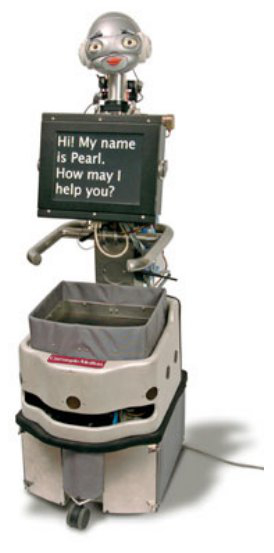
\includegraphics[width=\textwidth]{./img/pearl}
                \caption{Pearl}
                \label{fig:pearl}
        \end{subfigure}
        \begin{subfigure}[h]{0.45\textwidth}
                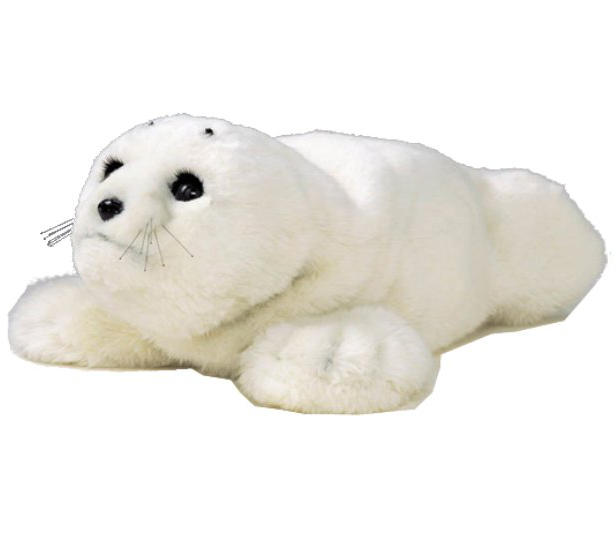
\includegraphics[width=\textwidth]{./img/paro}
                \caption{Paro}
                \label{fig:paro}
        \end{subfigure}
        \begin{subfigure}[h]{0.2\textwidth}
                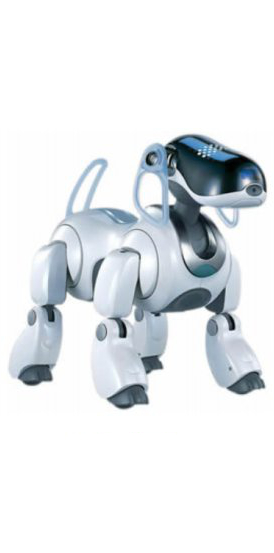
\includegraphics[width=\textwidth]{./img/aibo}
                \caption{Aibo}
                \label{fig:aibo}
        \end{subfigure}
        \caption{Service and companion robots for the elderly.}\label{fig:elder-robots}
\end{figure}

\emph{Paro} is a seal shaped companion robot used as medical therapy for the elderly (Figure~\ref{fig:paro}).
Since 2003, the work by Wada et al. provides a very good psychological and physiological evaluation of \emph{Paro}'s effects on the residents of a care house \cite{Wada2007,Wada2005,Wada2003}.
This robot contains a behaviour generation system that provides proactive, reactive and physiological reactions, such as, poses or motions, looking at the direction of a sound, and sleeping.
Their studies of both three weeks and one year have shown improvements in residents' moods, depression, stress levels, and social interactions with other residents.
The goal of such a robot is fully inspired in animal-assisted treatments, which have studied benefits in humans' health.
However, hospitals and health centres do not allow animals due to hygienic and safety reasons.
Hence, researchers found a great opportunity to build similar robotic animals.

Another example of a purely companion robot is the \emph{Huggable} \cite{Stiehl2005}, a teddy bear shaped covered of extremely sensitive touch sensors.
The \emph{Huggable} not only detects hard and soft touches, but also distinguishes between an object and a human touch.
Considering experiments in an hospital, this robot was connected to a computer in the nurses' station and allowed the staff to access the sensory input data.
Nurses could detect fear or insecurity by the way people hold the robot and provide appropriate assistance.

Purely companion robots in elderly care have only been applied to people with some kind of psychological or physiological disorder.
As a result, these studies have distinct target audiences and also different concerns when compared to the purposes of our proposed embodied agent.


\emph{Aibo} illustrates a robot that can be assigned to both the service type and the companion type (Figure~\ref{fig:aibo}).
It is considered by its creators as an entertainment type due to its puppy shaped body \cite{Fujita1983}, and its appearance tries to maintain a lifelike experience to its owners.
Tamura et al. started to study the acceptance and effects of this robot on elders with severe dementia \cite{Tamura2004}.
Their study revealed a relevant increase of social actions, emotions and feelings of comfort about past memories.


\begin{table}[h]
\centering
\caption{Robots for the aged population, their type and purposes}
\begin{tabular}{l|cccccc|}
\cline{2-7}
                                     & Pearl & RoboCare & Care-O-Bot-II & Paro & Huegable & Aibo \\ \hline
\multicolumn{1}{|l|}{Service type}   & \ding{51}     & \ding{51}        & \ding{51}             &      &          & \ding{51}    \\
\multicolumn{1}{|l|}{Companion type} &       &          &               & \ding{51}    & \ding{51}        & \ding{51}    \\ \hline
\multicolumn{1}{|l|}{Guidance}       & \ding{51}     & \ding{51}        & \ding{51}             &      &          &      \\
\multicolumn{1}{|l|}{Advice}         & \ding{51}     & \ding{51}        & \ding{51}             &      &          &      \\
\multicolumn{1}{|l|}{Therapy}        &       &          &               & \ding{51}    & \ding{51}        & \ding{51}    \\ \hline
\end{tabular}
\label{tab:elderly-robots}
\end{table}



Table~\ref{tab:elderly-robots} groups all the previously mentioned robots and their purposes.
This information strengthens the pertinence of our work, since existing robots for the elderly are focused on their physical and mental disabilities.
Providing pleasuring activities for the aged population, that are still capable of reasoning, should also be a concern.






\fancychapter{EMYS: the \emph{Sueca} player}
\label{chapter:approach}

Revising the purposes of this work, presented in Section~\ref{sec:goals}, the robotic agent that plays \emph{Sueca} has two main tasks: to choose an adequate card to play and to interact socially according to the game state.
In order to achieve these goals, some state-of-the-art approaches have been reviewed and considered for the implementation in our domain.
Thus the current chapter aims to carefully describe the decisions that were taken, some limitations imposed by the domain, as well as enhancements that have been made.
It starts with an overview of the whole system, proceeds with the implementation of the artificial player and last of all, details the development of the social agent.

\section{Architecture Overview}
\label{section:architecture_overview}

The model presented in Figure~\ref{fig:model} organises all the components involved in this system and their communications.
It considers a scenario where an embodied agent plays a physical card game against human players over a touch table.

\begin{figure}[ht]
  \centering
    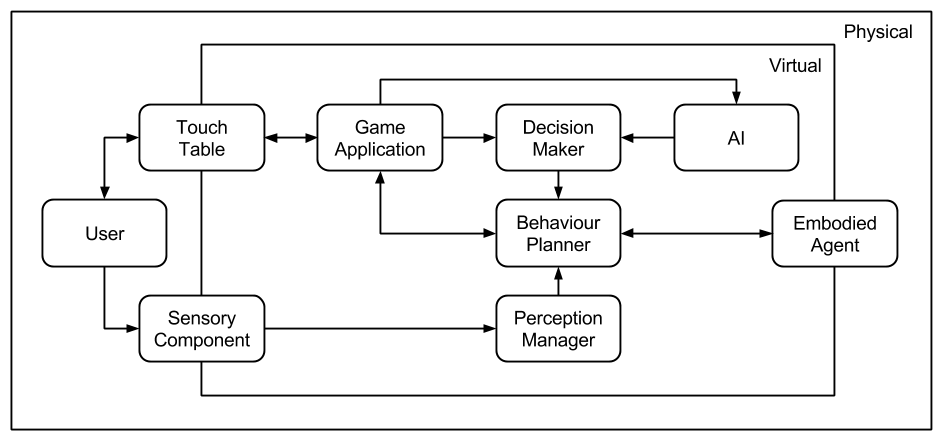
\includegraphics[width=1\textwidth]{./img/architecture}
  \caption{System architecture using components}
\label{fig:architecture}
\end{figure}

First of all, this model distinguishes physical components from virtual ones.
However, some entities are presented as both physical and virtual components and will not be detailed since their usage in this system did not demand any extensions for the scope of our domain (\emph{Touch Table}, \emph{Sensory Component} and \emph{Embodied Agent}).

The basic work-flow that illustrates the main functionalities of each component is as follows.
The human players, \emph{Users}, play with physical cards on top of a \emph{Touch Table}, and their game actions are managed by the \emph{Game Application} and communicated to both the \emph{\ac{ai}} and the \emph{Decision Maker}.
%\todo{check the sensory components!}
Besides their game actions, \emph{Users} also produce another sort of events that are captured by the \emph{Sensory Component} and handled by the \emph{Perception Manager}, for instance, face movements or the source direction of spoken interactions.
The \emph{\ac{ai}} includes all the reasoning about the game and decides the next move of the artificial player.
However, the \emph{Embodied Agent} will not only play a certain card, but will also include social behaviours.
As a result, the \emph{Decision Maker} balances the \emph{\ac{ai}} decisions and game information to produce an appropriate sequence of behaviours and inform them to \emph{Behaviour Planner}.
Lastly, the \emph{Behaviour Planner}, after receiving high-level intention-directed instructions, builds a suitable plan to execute the chosen instructions, considering the state of the \emph{Embodied Agent}, information from \emph{Perception Manager}, and additional game information from the \emph{Game Application}.

\begin{figure}[ht]
  \centering
    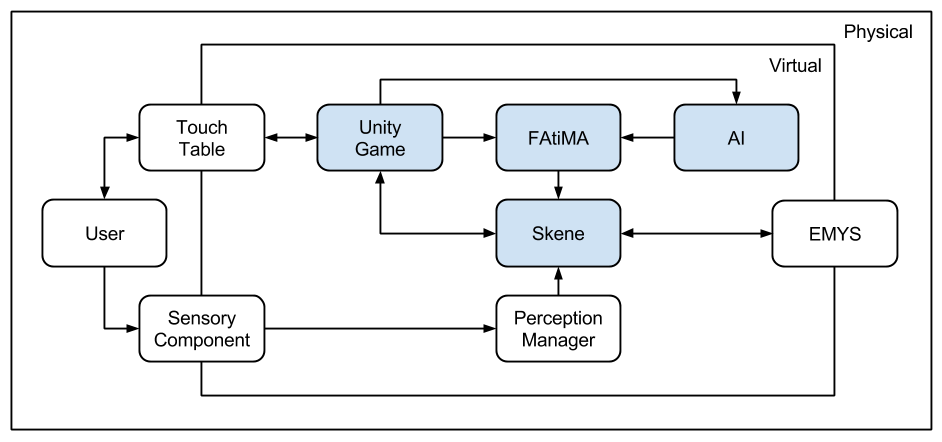
\includegraphics[width=1\textwidth]{./img/model}
  \caption{System architecture using modules}
\label{fig:model}
\end{figure}

%\todo{confirmar com o Tiago se sai uma seta do skene para o unity!!!}
The previously described architecture is instantiated as shown in Figure~\ref{fig:model} and the blue modules are thalamus communicating entities.
This concept arises from the Thalamus Framework \cite{Ribeiro}, which enables the usage of entities that can be registered at runtime in a server in order to send and receive specific messages.
These entities are publishers and subscribers of the channels they want to write on and listen to, respectively.
The implementation provided by this framework works by simply inherit from the \emph{ThalamusClient} class and implement the interfaces of the messages that the entity wants to exchange.

The \emph{Unity Game} module is responsible for displaying the interface of the game, reading the physical cards, publishing all the relevant game events and subscribing to the plays of artificial players.

The chosen \emph{Behaviour Planner} is \emph{Skene} \cite{Ribeiroa}, which tightens the communication between the world and an embodied agent with a high-level behaviour description language, also known as utterances.
These utterances might include instructions for gazing, pointing, animating or sound, among other things.
Additionally, considering some instructions require target positions or other game information, Skene subscribes to \emph{Unity game} messages to keep that information updated.

The \emph{\ac{ai}} and \emph{FAtiMA} modules answer to our primary goals, for that reason, their implementations are carefully detailed in Section~\ref{sec:artificial_player} and Section~\ref{sec:behaviour_planner}, respectively.

\section{An intelligent player}%The artificial player}
\label{sec:artificial_player}

This section will describe the most relevant implementation details of the artificial player.
After thoroughly analysing state-of-the-art techniques to solve imperfect information games, and considering \emph{Sueca} is, at this moment, computationally unsolved, the chosen approach was \ac{pimc}.
To implement this search technique, there are three key concepts or algorithms that require a full understanding: the Information Set, the PICM Search and the MinMax Algorithm.

\subsection*{Information Set}

An information set represents all the visible information during a game, and also inferred information based on certain events.
The player must keep an instance of the information set per game and update it when necessary.
It stores the known hand of the player and a deck with all the cards whose owner is unknown.
As result, each time another player plays a card, it should be removed from that deck.

The purpose of managing unplayed cards is to sample possible card distributions for the other three players with their real conditions.
These sampled distributions will be used during the \ac{pimc} search and the closer they are to the real world, the better the search returning value will be.
Additionally, the information set keeps track of suits per player and, when a player does not follow the leadsuit of a trick, it removes that suit from the player possible suits.
By possessing this information, sampling the distributions gets closer to the world, however it increased the complexity of the sampling process.
The method builds a \ac{csp} where:
\begin{itemize}
\item variables are the unplayed cards;
\item each domain is the set of players that still have that suit;
\item and the constraints are the number of times a player can be assigned to a card.
\end{itemize}


\subsection*{\ac{pimc} Search}

The following pseudo-code of the \ac{pimc} search algorithm guided the implementation.
To recapitulate the main point of this algorithm, considering it can choose up to \#Moves($I$), it samples $N$ possible card distributions for the other three players and calculates the reward of playing each possible move for the $N$ sampled worlds. The returned move is the one that gave more accumulated reward.

\begin{algorithm}
	\caption{PIMC search algorithm}
	\begin{algorithmic}[1]
		\Procedure{PIMC}{InfoSet $I$, int $N$}
			\ForAll {$m \in$ Moves($I$)}
				\State $val[m]$ = 0
			\EndFor
			\ForAll {$i \in \{ 1..N\}$}
				\State $x$ = Sample($I$)
				\ForAll {$m \in$ Moves($I$)}
					\State $val[m]$ += PerfInfoValue($x$, $m$)
				\EndFor
			\EndFor
			\State \textbf{return} $\underset{m}{argmax}\{ val[m] \}$
		\EndProcedure
	\end{algorithmic}
\end{algorithm}


\subsection*{MinMax Algorithm}

Bla bla bla


\subsection{Drawbacks}

Bla bla bla


\subsection{Enhancements}

Bla bla bla

\section{A cooperative and non-cooperative player}%Behaviour Planner Component}
\label{sec:behaviour_planner}

Robot has been implemented...


\clearpage


\fancychapter{Results and discussion}
\label{chapter:results}

\section{User Centred Studies} \label{sec:user-studies}

Developing a robot for aged people brings some delicate questions.
The potential users sometimes have few, or nonexistent, experience with technology, which makes it is difficult for them to understand how robots work and what they can actually do.
As a result, understanding their needs, expectations, and fears is another concern \cite{Oliveira}.


The current section explains the methodology, procedures and preliminary results of an already developed user study in a care home.
It involved two different activities, a focus group and a pilot card game study, as a result of two distinct motivations: to understand the elderly' concerns about robots, and to analyse the set-up to further collect information in the game domain.
%This aimed to collect specific social, verbal and nonverbal behaviours, and also some cognitive and strategic guidelines in the domain of \emph{Sueca}.
%Additionally, another goal of these user studies is to understand their needs, expectations, and fears \cite{Oliveira}. As a result, the following pilot study was developed in a care home in order to answer all these questions.






\subsection{Focus Group}

A focus group seems to be a good approach for a first meeting due to the informal and conversational way of interacting with participants.
The goal of this activity was to introduce to the elderly the robots' theme, and to understand their opinions and expectations.
To accomplish this purpose, used techniques were a Brainstorming and a Storytelling.

\subsubsection{Methodology}
The elderly participants were divided into groups of 5.
There were 2 researchers per group commanding and guiding all the process.
The list of materials used, per group:

\begin{itemize}
\item An illustrative video of existing robots;
\item 6 photographs of different robots, including 3 of service type and 3 of companion type (Paro, EMYS, Pleo, Pearl, PR2, and Care-O-Bot);
\item Two white boards and three pens (black, red and green);
\item Three hypothetical stories of robots;
\item An audio recorder;
\item Four lavalier microphones;
\item A video camera.
\end{itemize}

The last three items will only be used for a further analysis of this focus group.
The video tries to answer the questions: what is a robot, what can robots do, how do they work, do they fail and how do science fiction movies present robots to us.
In order not to bias their thoughts, we tried to gather positive and negative aspects of existing robots.
The three hypothetical stories aim to bring ethical discussions to the focus group \cite{Kahn2006,Should2010}.
For instance, an elderly that owns a robot in his home tells him a secret.
If that robot is questioned about the secret, should it or should it not tell other people the truth?

\subsubsection{Procedures}
All the materials enumerated in the previous list were arranged as in Figure~\ref{fig:focus-group}.
Firstly, each person in the room briefly introduces himself in order to make everyone feeling more comfortable.
Secondly, the video is shown.
Then, everyone starts discussing about robots' purposes and they are registered in one of the white boards with the black coloured pen.
People also express a positive or negative impression of each robot's purpose and their opinions decide the colour of the surrounding line (Appendix).
For instance, the sentence ``Call an ambulance'' written on the board is surrounded by a green line if they think it is a good purpose for a robot.
After finishing this task, one of the group leaders writes all the sentences previously collected in the second board but without the surrounding green or red lines.
The other group leader starts reading the hypothetical stories and opens a new discussion about what the robots of each story should do.
He also presents the photographs and tries to understand which robot is more suitable for each purpose in their opinion.
When bringing the new board to the room, the idea is to understand if their positive and negative opinions about each purpose have changed.


\subsubsection{Preliminary Results}

This focus group is an ongoing activity that has not yet been fully analysed.
Information has already been collected from 3 different focus groups with a sum of 15 participants.
For instance, contrasting with what was expected, the elderly do not feel uncomfortable and disrespected with a robot calling the doctor and revealing improper behaviours about its owner (e.g. a diabetic elder eating a chocolate cake slice).
Instead, they think it is a valuable aid in their lives and might save them while disrespecting strict instructions.
In addition, their safety is their prior worry, and when walking through the house and sometimes due to physical disabilities, they fear about falling and not being noticed.




\begin{figure}
        \centering
        \begin{subfigure}[h]{0.49\textwidth}
                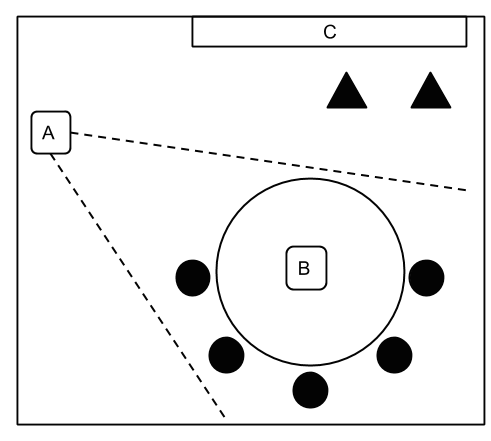
\includegraphics[width=\textwidth]{./img/focusGroup}
                \caption{Focus Group}
                \label{fig:focus-group}
        \end{subfigure}
        \begin{subfigure}[h]{0.49\textwidth}
                
\includegraphics[width=\textwidth]{./img/cardGame}
                \caption{Card game}
                \label{fig:card-game}
        \end{subfigure}
        \caption[Setting of the user study activities.]{Setting of the user study activities. \textbf{A} - Video recorder \textbf{B} - Audio recorder / Microphone \textbf{C} - White board \textbf{D} - cards \ding{108} - Aged person \ding{115} - Group leader}\label{fig:user-studies}
\end{figure}





\subsection{Card Game}
%Considering the goal of developing a social embodied agent in a game scenario, user studies will be further required, similarly to what Pereira et al. have done with the Risk player.

A pilot card game activity with the elderly aims two distinct purposes.
On one hand, to collect all kind of behaviours and interactions between players during the game.
On the other hand, to rehearse and check the technical set-up for further studies.
It is important to understand difficulties, for instance, lightning conditions might affect video recording, or the room acoustic and noise might affect audio recording.
Testing these conditions is essential to guarantee the analysis of additional studies.
Moreover, this activity aims to perceive how the elderly play, what they say and how they behave in certain game states.

\subsubsection{Methodology}
Recording each \emph{Sueca} card game requires four players, a card deck, a table and chairs for the four players, two video cameras and an audio recorder with four microphones.

\subsubsection{Procedures}
All the previously enumerated material was arranged as in the Figure~\ref{fig:card-game}.
Each video camera was positioned to capture the hands of two adjacent players.
Players were recorded during a tournament of several games.
They were told to play as long as they wanted with a maximum duration of one hour.

\subsubsection{Preliminary Results}
The session took only 40 minutes, since the 4 players were feeling weary.
Ten games, with an average duration of 3,75' each, were collected.
From the average duration, 1' belongs to the initial setting of shuffling, distributing, and rearranging the cards in each hand.
The points per team were being counted during the game.

As expected, players did not frequently talk during the game.
\emph{Sueca} is indeed traditionally called a silent game.
After a game, paired players frequently discuss extremely good or bad moves from each other.
However, the analysis was focused mostly on interactions during the game.
Table~\ref{tab:interactions} illustrates the collected expressions, the game stage and its intention.
Considering players said specific domain words, expressions were not translated in order not to lose their meaning and regarding the future usage of these sentences in a Portuguese environment.


\begin{table}
\caption{Examples of expressions collected during the card game activity and its respective classification.}
\resizebox{\textwidth}{!}{%
\begin{tabular}{|l|m{0.3\textwidth}|m{0.3\textwidth}|}
\hline
\textbf{Expression} & \textbf{Game Stage} & \textbf{Intention} \\ \hline
\textit{Joga }{[}player-name{]}\textit{!} & Before a play & Speed up a play. \\ \hline
\textit{Anda }{[}player-name{]}\textit{!} & Before a play & Speed up a play. \\ \hline
\textit{Podes jogar, }{[}player-name{]}\textit{!} & Before a play & Speed up a play. \\ \hline
\textit{Quase que livr\'amos.} & After collecting the first points & Hopeful or ironic comment. \\ \hline
\textit{E eu puxo trunfo.} & Initialising a turn with a trump card & State an action. \\ \hline
\textit{Outro trunfo!} & Play a trump card after an already played trump card & State an action. \\ \hline
\textit{Outro(a) }{[}suit{]}\textit{!} & Play a {[}suit{]} card after an already played {[}suit{]} card & State an action. \\ \hline
\textit{O trunfo \'e }{[}suit{]}\textit{.} & Anytime & Give game information. Answer a question. \\ \hline
\end{tabular}
}
\label{tab:interactions}
\end{table}


Regarding the video recording, a relevant aspect that has been noticed was the lighting reflection through the cards.
If this technique will be adopted to collect game play information, lighting conditions should be well prepared.


%Additional cues will be evaluated 

\clearpage



\fancychapter{Conclusions}
\label{sec:conclusion}

\section{Conclusion}
My conclusions are...

\section{Future work}
Some future work might be...


\bibliography{references}{}
%\bibliographystyle{plainnat}
\cleardoublepage

%\appendix
%\cleardoublepage
\fancychapter{Appendix A - Approach supplementary material}
\label{sec:appendix_a}

\thispagestyle{empty}

\begin{landscape}
    \begin{table}[htb]
    \centering
     \begin{threeparttable}
     \caption{Plant miRNA target prediction tools, adapted from~\citet{Srivastava2014}}
     \label{tbl:tool_comparison}
     \begin{tabular} {c c c c c c c l c} \toprule
     Name & Comp\tnote{1} & Cons\tnote{2} & Acc\tnote{3} & Mul\tnote{4} & Func\tnote{5} & Code & Link & Ref\tnote{6} \\ \hline
     Patscan & \checkmark & & & & & & {\scriptsize N/A} & \cite{Dsouza1997} \\
     miRNAssist & \checkmark & & & \checkmark & & & {\scriptsize N/A} & \cite{Xie2007} \\
     miRU & \checkmark & \checkmark & & & & & {\scriptsize N/A} & \cite{Zhang2005} \\
     WMD3 & \checkmark & & \checkmark & & & & {\scriptsize \url{http://wmd3.weigelworld.org/}} & \cite{Ossowski2008} \\
     TAPIR & \checkmark & \checkmark & \checkmark & & & \checkmark & {\scriptsize \url{http://bioinformatics.psb.ugent.be/webtools/tapir/}} & \cite{Bonnet2010} \\
     UEA sRNA & \checkmark & & \checkmark & & & & {\scriptsize \url{http://srna-tools.cmp.uea.ac.uk/plant/}}\tnote{7} & \cite{Moxon2008} \\
     Target-align & \checkmark & & & & & \checkmark & {\scriptsize \url{http://www.leonxie.com/}} & \cite{Xie2010} \\
     Targetfinder & \checkmark & \checkmark & \checkmark & & & \checkmark & {\scriptsize \url{http://carringtonlab.org/resources/targetfinder}} & \cite{Fahlgren2007} \\
     p-TAREF & \checkmark & \checkmark & \checkmark & & & \checkmark & {\scriptsize \url{http://scbb.ihbt.res.in/new/p-taref/form1.html}} & \cite{Jha2011} \\
     psRNATarget & \checkmark & & \checkmark & \checkmark & \checkmark & & {\scriptsize \url{http://plantgrn.noble.org/psRNATarget/}} & \cite{Dai2011a} \\
     imiRTP & \checkmark & \checkmark & \checkmark & \checkmark & \checkmark & & {\scriptsize \url{http://admis.fudan.edu.cn/projects/imiRTP.htm}}\tnote{7} & \cite{Ding2011} \\ \bottomrule
      \end{tabular}
      \begin{tablenotes}
        {\scriptsize  Note: \item[1] Complementarity; \item[2] Conservation; \item[3] Accessibility; \item[4] Multiplicity; \item[5] Functionality; \item[6] Reference \item[7] Currently offline}
      \end{tablenotes}
     \end{threeparttable}
    \end{table}
\end{landscape}

\begin{figure}[H]
\begin{lstlisting}[language=bash]
#!/bin/sh

cd "$(dirname "$0")"

TARBASE=validated_targets_tarbase.csv

#generate a processed miRNA file
sed 's/ .*//g' mirna_unprocessed.fa > mirna.fa

sed -re '/ath-/!d' ../tarbase_data.csv > temp 

cut -f2,4 temp | awk '{$2=toupper($2)}1' | sed 's/ /,/g' | sed 's/mir/miR/g'| awk -F, '{print $2,$1}' OFS=, > $TARBASE

cat  validated_targets_* | sort | uniq > validated_targets.csv

rm temp
rm $TARBASE
	
\end{lstlisting}
\caption{Script for preprocessing miRNA and validated targets datasets}
\label{scr:datasets}
\end{figure}

\begin{figure}[H]
\begin{lstlisting}[language=bash]
#!/bin/sh

cd "$(dirname "$0")"

#processing psRNATarget targets
sed "/#/d" psRNATarget/unprocessed_targets.txt | cut -f1,2  | tail -n +2 | sed 's/\t/,/g' | awk -F, '{print $2,$1}' OFS=, | sort | uniq > psRNATarget/processed_targets.csv

#processing TAPIR targets 
sed -e "/#/d" tapir/unprocessed_targets.txt -re '/miRNA |target /!d' -e 's/([[:space:]])+/\t/g' | cut -f2 | paste - - -d"," |  tr ' ' ',' | awk -F, '{print $2,$1}' OFS=, | sort | uniq > tapir/processed_targets.csv

cat psRNATarget/processed_targets.csv tapir/processed_targets.csv validated_targets.csv | sort | uniq  > subset.csv
\end{lstlisting}
\caption{Script for pre-processing the results from tools}
\label{scr:tools}
\end{figure}

%\cleardoublepage
\fancychapter{Appendix B - {\sc Pinetree} documentation}
\label{sec:appendix_b}

\includepdf[pages={-}]{appendix_b/user_guide.pdf}

\thispagestyle{empty}



\end{document}